\subsubsection{Sweep-Verfahren}
\label{ssub:voronoiAlgorithmsSweep}
Grundsätzlich funktioniert das Sweep-Verfahren so, dass man eine bestimmte Eigenschaft einer Menge von Objekten ermitteln möchte. Dazu werden alle Objekte der Reihe nach besucht und für alle bereits besuchten Objekte werden geeignete Informationen (welche je nach Anwendungsfall variieren) abgelegt. Aus den Informationen ergibt sich schlussendlich die gesuchte Eigenschaft.

Um den Sweep-Algorithmus auf ein Voronoi-Diagramm anwenden zu können, werden beim Sweepen nur die Teile des Voronoi-Diagramms gespeichert, welche links der Sweep-Line $L$ liegen und sich nicht mehr ändern können. Dies heisst, dass kein Punkt rechts von $L$ das Gebiet links der Sweep-Line beeinflusst. Konkret werden die $n$ Punkte aus $S$ in der Reihenfolge aufsteigender X-Koordinaten sortiert und dann jeweils der \gls{bisector} zwischen einem Punkt aus $S$ und der Sweep-Line $L$ in Form einer Parabel $B(p_j, L)$ gebildet. Dies ergibt schlussendlich den Rand der Voronoi-Region, bestehend aus Parabelbögen, genannt \textit{\textbf{Wellenfront}} $W$. Die Parabeln folgen dabei der Sweep-Line mit halber Geschwindigkeit~\parencite[S. 288]{klein2005algorithmischegeometrie}.

Der Schnittpunkt zweier benachbarter Stücke der Wellenfront $W$, z.B. $B(r, L) \cap B(s, L)$, rückt mit fortschreitender Sweep-Line längs deren geraden Bisektors $B(r, s)$ vor. ``Die Verlängerung dieser Bisektoren nach rechts über die Wellenfront hinaus werden \textbf{\textit{Spikes}} genannt'' definiert~\citeauthor{klein2005algorithmischegeometrie} (\citeyear[S. 289]{klein2005algorithmischegeometrie}).

Mit Fortschreiten der Sweep-Line ist es natürlich möglich, dass ein Wellenstück verschwindet, da es den Schnittpunkt seiner beiden Spikes erreicht, und, dass ein neues Wellenstück erscheint, wenn die Sweep-Line $L$ auf einen neuen Punkt $p$ aus $S$ trifft.

Um schlussendlich das Voronoi-Diagramm $V(S)$ von $S$ zu bilden, wird $V(S)$ von Ereignis zu Ereignis erweitert. Wenn kein Ereignis mehr zu bearbeiten ist, wird die Sweep-Line entfernt und alle noch vorhandenen Spikes werden als unbeschränkte Voronoi-Kanten zu $V(S)$ hinzugefügt~\parencite[S. 289 bis 291]{klein2005algorithmischegeometrie}.

Wird eine möglichst effiziente Datenstruktur zur Speicherung des Voronoi-Diagramms $V(S)$, wie etwa die Sweep-Status-Struktur und die Ereignis-Struktur wie von~\citeauthor{klein2005algorithmischegeometrie} vorgeschlagen, bleibt die Grösse in $O(n)$ und die Laufzeit $O(n \log(n))$ (\citeyear[S. 294]{klein2005algorithmischegeometrie}).

\newpage{}

Folgende Darstellungen\footnote{Eigene Darstellung mittels Geogebra} zeigen das Fortschreiten der Sweepline und die Entsteheung einer Voronoi-Kante:

\begin{minipage}[t]{0.5\textwidth}
    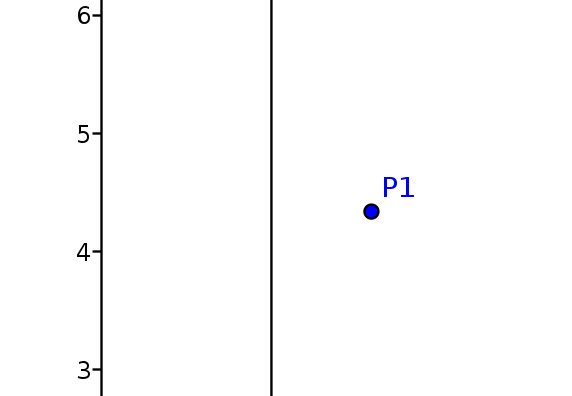
\includegraphics[width=\textwidth]{images/sweep_line_01.png}
    \captionof{figure}{Sweepline ``vor'' Punkt $P1$}
\label{fig:delaunayExample01Orig}
\end{minipage}
\begin{minipage}[t]{0.5\textwidth}
    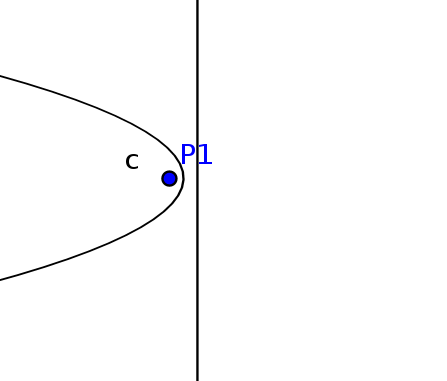
\includegraphics[width=\textwidth]{images/sweep_line_02.png}
    \captionof{figure}{Sweepline ``nach'' $P1$ mit Bisektor $B(P1, L)$}
\label{fig:delaunayExample01500}
\end{minipage}

\begin{minipage}[t]{0.5\textwidth}
    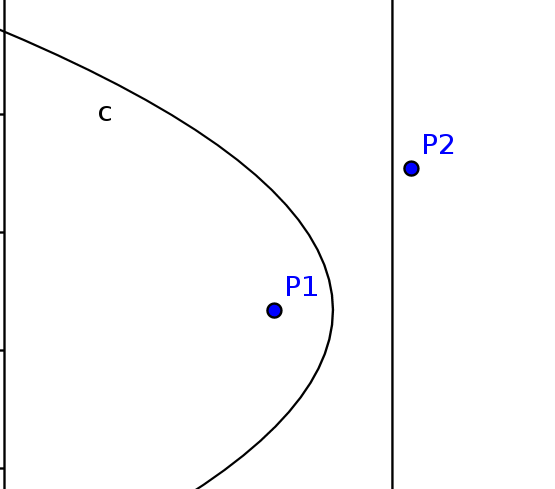
\includegraphics[width=\textwidth]{images/sweep_line_03.png}
    \captionof{figure}{Sweepline ``nach'' $P1$, ``vor'' $P2$}
\label{fig:delaunayExample018000}
\end{minipage}
\begin{minipage}[t]{0.5\textwidth}
    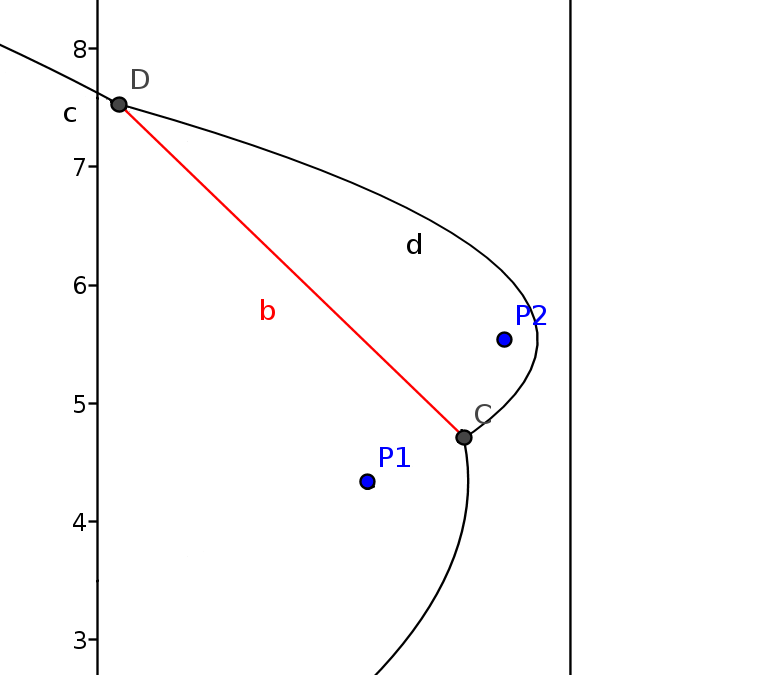
\includegraphics[width=\textwidth]{images/sweep_line_04.png}
    \captionof{figure}{Sweepline ``nach'' $P1$ und $P2$ mit Voronoi-Kante $b$}
\label{fig:delaunayExample018000}
\end{minipage}
